\section{Introduction}
We were working with Zebra during the first sprint. Zebra is now called `Sekvens' in the GIRAF application. `Sekvens' is an application that allows the guardians of autistic children, to present sequences of pictograms to an autistic child. This aids the autistic children in performing daily routines, which they would not be capable of without a visualization. The sequences made for the autisctic people are various, but could be e.g. a sequence for how to wash hands, how to put on outdoor clothing during winter, or how to behave during dinner when they sit and eat their packed lunch. The sequence application is a digital solution to an existing analog solution which they currently use in institutions in and near the city of Aalborg.

\begin{figure}
\centering
\begin{minipage}{.7\textwidth}
\centering
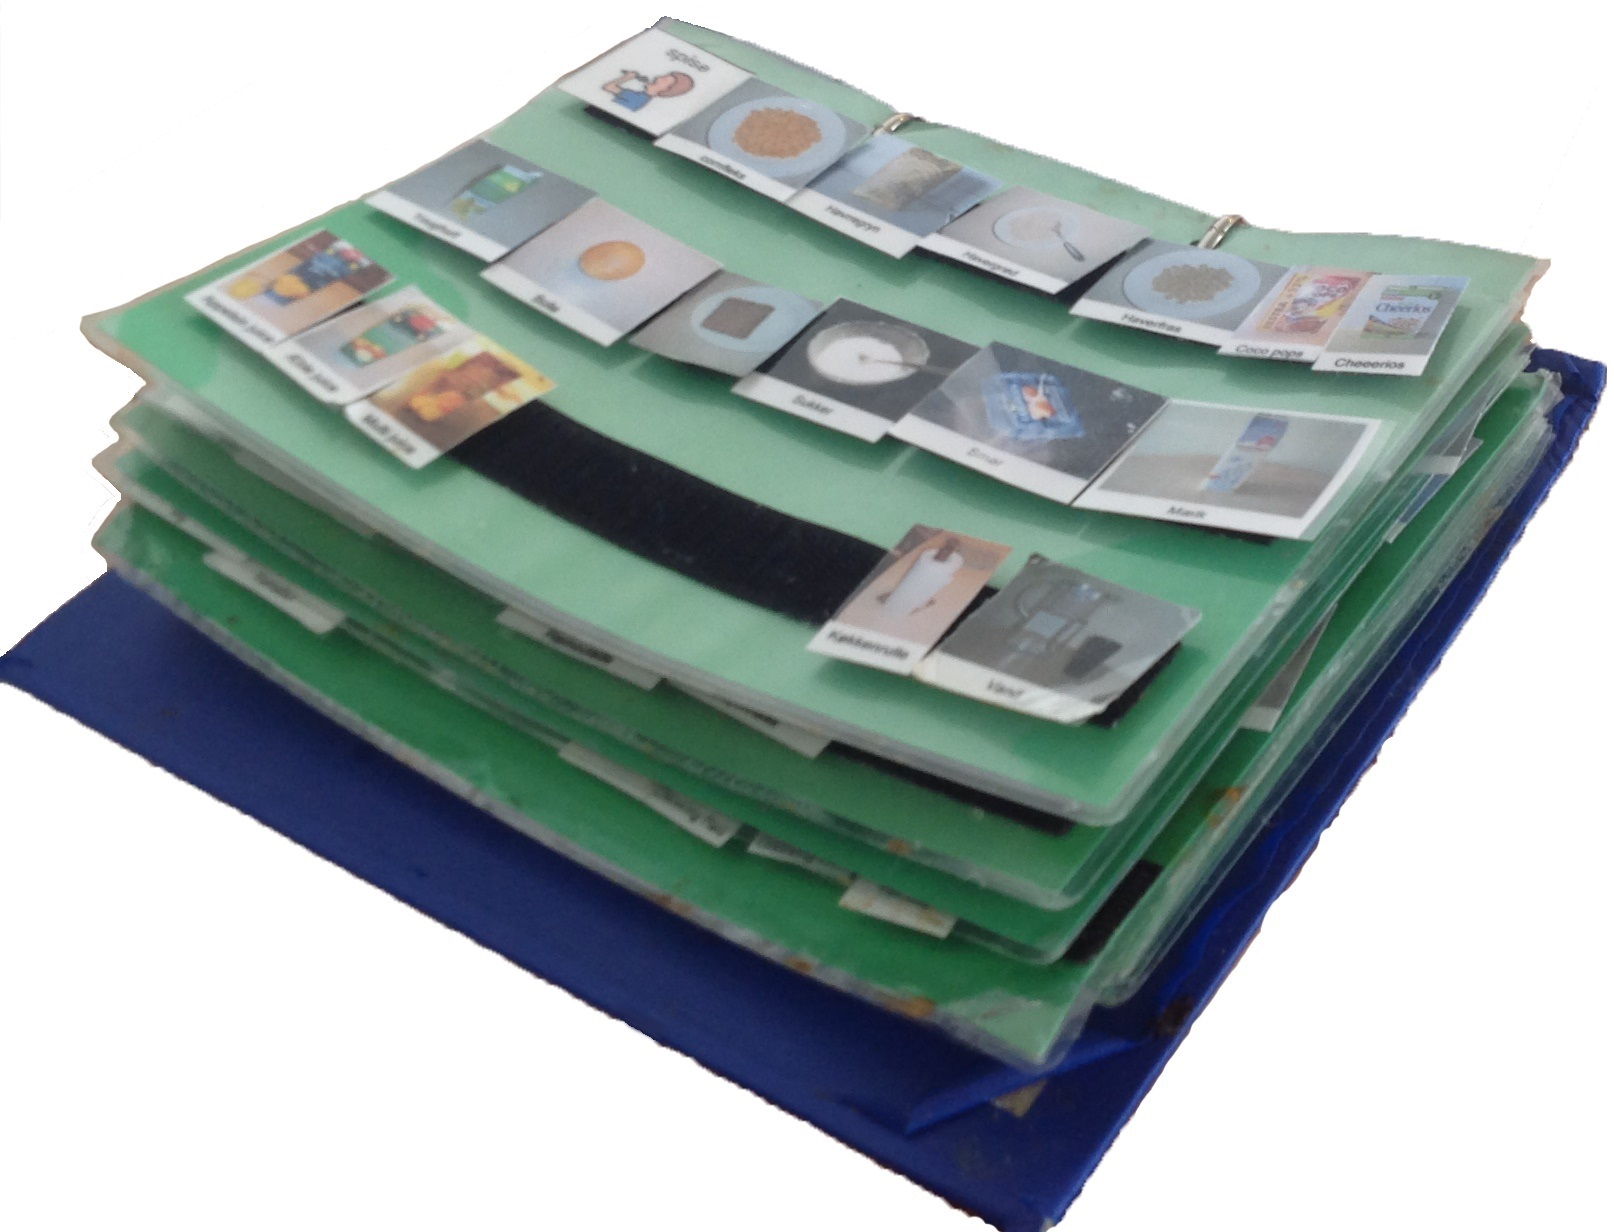
\includegraphics[scale=0.17]{Pics/Sprint1/pictogram_binder.jpg}
\caption{A pictogram binder with already constructed sequences}
\label{fig:pictogram_binder}
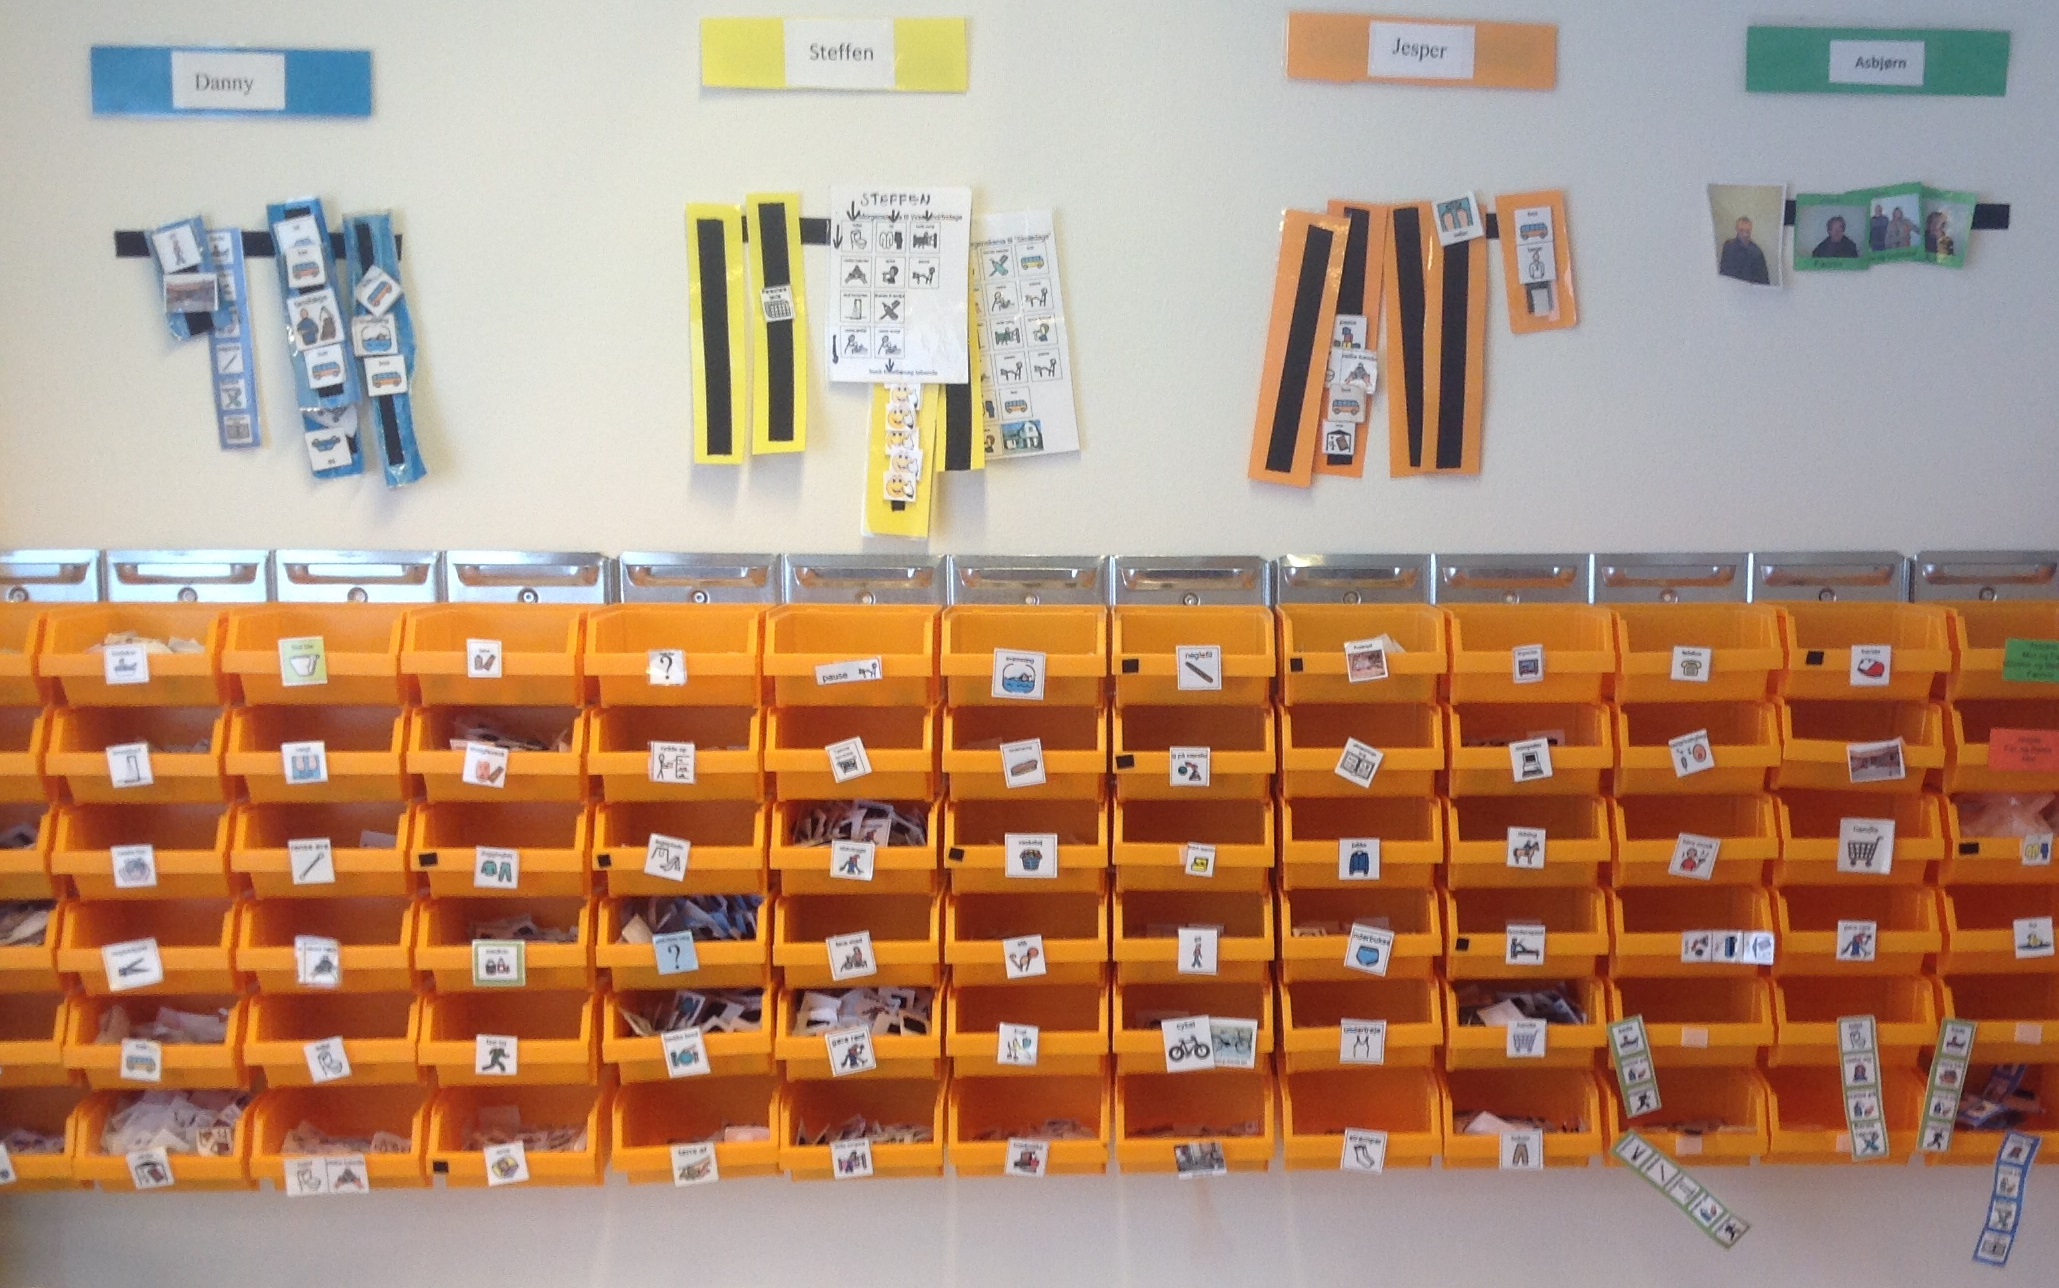
\includegraphics[scale=0.14]{Pics/Sprint1/pictogram_containers.jpg}
\caption{Pictogram containers and personal sequences for the children}
\label{fig:pictogram_container}
\end{minipage}\hfill
\begin{minipage}{.3\textwidth}
\centering
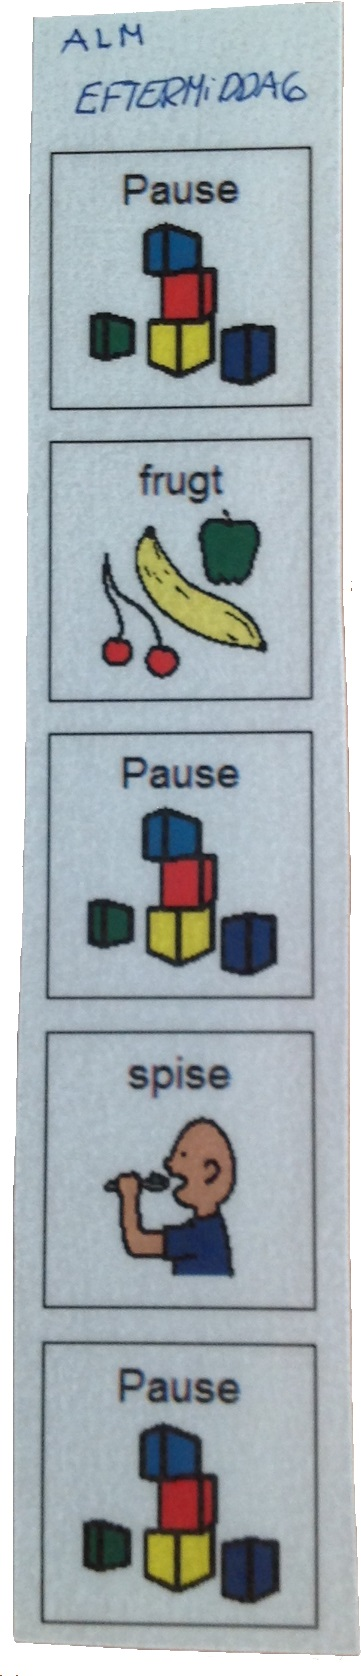
\includegraphics[scale=0.17]{Pics/Sprint1/pictogram_sequence.jpg}
\caption{A sequence of pictograms made for eating an afternoon meal}
\label{fig:sequence}
\end{minipage}
\end{figure}

It is quite obvious, that the current solution is exhaustive (An example of a current solution is portrayed in figure \ref{fig:pictogram_binder},\ref{fig:pictogram_container} and \ref{fig:sequence} ). It was previously decided by a group of software students on 6th semester, to work on a digital solution. They created a first draft of the application that we a year later picked up and continued to work on. They had an application up and running, but had remaining issues and obstacles they did not have time to solve.

During the first sprint, we had a goal to solve the remaining issues and obstacles for the Sequence application. We focused on making the current application work instead of developing new features or creating additional functionality to the application. This was a common agreement among the software 6 students working on the multi-project




